\problemname{Mini Golf}

\begin{center}
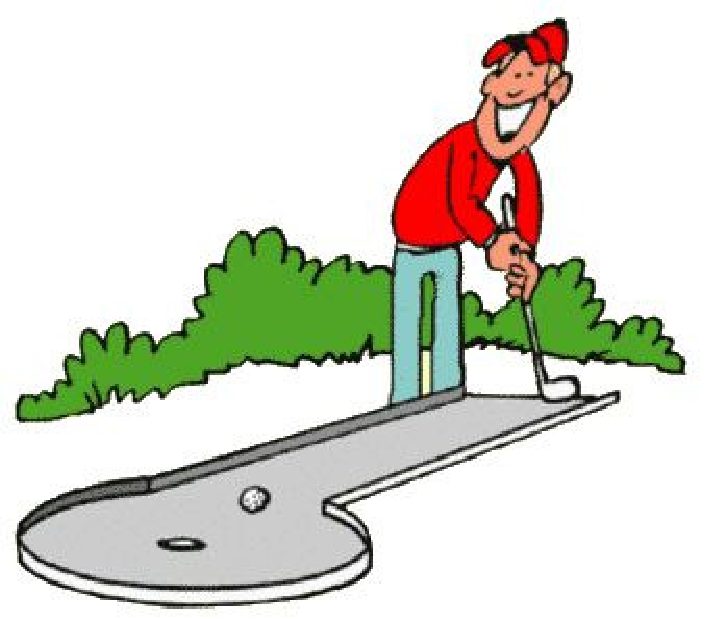
\includegraphics[width=0.3\textwidth]{minigolfbild.pdf}
\end{center}

A mini golf course has $N$ holes. Every other hole (odd numbers) is so-called ``{\em par 2}'' and
every other (even numbers) is ``{\em par 3}'', where ``{\em par}'' is the recommended number of strokes a golfer should
complete a certain hole in. There is also a rule that if you take more than $7$ strokes on a hole, it still only
counts as $7$ strokes in the tally.

Write a program that, given the number of strokes you used on each hole, calculates the total result over/under par.

\section*{Input}
First a line with an integer $N$ $(2\le N\le 10)$, the number of holes. Then follows a line with $N$ integers between $1$ and $10$ each: the number of strokes you used on each hole.

\section*{Output}
One line with one integer, the total result over/under par.

\section*{Scoring}
Your solution will be tested on a set of test groups.
To earn points for a group, you must pass all test cases in that group.

\noindent
\begin{tabular}{| l | l | l |}
\hline
  Group & Points & Constraints \\ \hline
  $1$    & $40$       &  No hole took more than 7 strokes to complete.  \\ \hline 
  $2$    & $60$       &  No additional constraints. \\ \hline
\end{tabular}

\section*{Explanation of Samples}

\begin{figure}[!htb]
\minipage{0.5\textwidth}
{\bf Sample 1:}\\
\begin{tabular}{||l|c|c|c||c||}\hline \hline
Hole & 1 & 2 & 3 & Total \\ \hline \hline
Par & 2 & 3 & 2 & 7 \\ \hline 
Strokes & 5 & 3 & 1 & 9 \\ \hline
+/- & +3 & 0 & -1 & +2 \\ \hline \hline
\end{tabular}
\endminipage\hfill
\minipage{0.5\textwidth}
{\bf Sample 2:}\\
\begin{tabular}{||l|c|c|c|c|c|c||c||}\hline \hline
Hole & 1 & 2 & 3 & 4 & 5 & 6 & Total \\ \hline \hline
Par & 2 & 3 & 2 & 3 & 2 & 3 & 15 \\ \hline 
Strokes & 1 & {\bf 7} & 1 & 1 & 1 & 1 & 12 \\ \hline
+/- & -1 & +4 & -1 & -2 & -1 & -2 & -3\\ \hline \hline
\end{tabular}\\
(note that the 9 strokes on the second hole are recorded as 7)
\endminipage\hfill
\end{figure}
